\documentclass[12pt]{article}

\usepackage{sbc-template}
\usepackage{graphicx,url}
\usepackage[brazil]{babel}
\usepackage[utf8]{inputenc}
\usepackage{float}
\usepackage{setspace}

\usepackage{tabularx}
\usepackage{cite}

\begin{document}
\sloppy
\singlespacing
\title{Mezuro - Coleta, interpretação e exibição automatizadas de métricas estáticas de código-fonte}

\author{Rafael R. Manzo\inst{1}, Diego de A. M. Camarinha\inst{1},\\
        Alessandro Palmeira\inst{1}, Fellipe S. Sampaio\inst{1},\\
        Renan Fichberg\inst{1}, Paulo Meirelles\inst{2}}

\address{Instituto de Matemática e Estatística -- Universidade de São Paulo (USP)\\
  Rua do Matão, 1010 -- 05508-090 -- Cidade Universitária -- São Paulo -- SP -- Brasil
\nextinstitute
  Faculdade de Engenharia -- UnB Gama (FGA)\\
  Gama -- DF -- Brasil
  \email{manzo@ime.usp.br,\{diego.camarinha,alessandro.palmeira\}@usp.br}
  \email{\{renan.fichberg,fellipe.sampaio\}@usp.br,paulo@softwarelivre.org}
}

\maketitle
\begin{abstract}
  In this article, we present the motivation, main characteristics, architecture and a use case of the Mezuro free software project.
  The motivation behind the project will be presented through the problem of analyzing code metrics, making a brief comparison with
  other solutions avaliable in the market.
  We enumerate the main characteristics that distinguish Mezuro from its competitors and why its use can be more advantageous compared to other
  web services for source code analysis.
  \\*
  \textbf{Keywords:} free software, source code analysis, source code metrics, web services.
\end{abstract}

\begin{resumo}
  Neste artigo, apresentaremos a motivação, as principais características, arquitetura e um caso de uso do projeto de software livre Mezuro.
  A motivação por trás do projeto será apresentada por meio da problemática da análise de métricas de código, fazendo um breve
  comparativo com outras soluções disponíveis no mercado. Enumeraremos as principais características que diferenciam
  o Mezuro de seus concorrentes e porque seu uso mostra-se mais vantajoso em comparação a outros serviços web de análise de código-fonte.
  \\*
  \textbf{Palavras-chave:} software livre, análise de código fonte, métricas de código, serviços web.
\end{resumo}

\newpage

\section{Introdução} \label{sec:intro}
Métricas de código-fonte (ou mais geral, de software) estático são medidas extraídas a partir das análises léxica e sintática do código-fonte de um programa sem compilá-lo ou executá-lo e podem ser primitivas ou compostas (composição de uma ou mais métricas primitivas) \cite{m13}. Sua principal função é fornecer informações sobre complexidade, compreensão, testabilidade, manutenibilidade e evolução do código\cite{m13}.

Exemplos de métricas podem ser simples como linhas de código (\textit{loc - lines of code}) e quantidade de métodos por classe, ou complexas como conexões aferentes de uma classe (\textit{acc - afferent connections per class}).
Hoje, existem diversas ferramentas para a simples extração de métricas, como pylint (Python), metric\_fu (Ruby) e Analizo (C/C++ e Java), cada uma com diferentes graus de usabilidade, padrões e conjuntos de métricas, tornando estas importantes informações inacessíveis para muitos usuários.

\section{Motivação}
Por meio da avaliação de métricas de código-fonte podemos definir como está a qualidade do software e pensar em estratégias interessantes para lidar com a chamada ``crise do software'' \cite{nr68}. Esta afirma que, com o crescimento da capacidade computacional, mais problemas difíceis se tornam viáveis para serem resolvidos, mas que, por outro lado, a complexidade dos equipamentos (\textit{hardware}) e do processo de desenvolvimento atuais combinados com a complexidade dos problemas exacerbam falhas do software. Assim, controlar a qualidade com que um software evolui durante o tempo torna-se uma ferramenta para se identificar e prevenir tais falhas.

Porém, incorporar esta avaliação às metodologias de desenvolvimento de software não pode ser um processo manual, caso contrário corre-se o risco de cair em desuso. Isto pois as ferramentas de extração de métricas em geral não apresentam uma interface amigável para seres humanos lerem seus resultados e muito menos um padrão entre si.
Neste contexto, uma ferramenta com as seguintes características se faz necessária para a introdução deste tipo de avaliação constante às metodologias:
\begin{itemize}
  \item interface que agrupe as diversas ferramentas disponíveis hoje no mercado
  \item permita seleção e composição de métricas de forma flexível
  \item manutenção de um histórico de evolução
  \item exiba os resultados de forma amigável
\end{itemize}
Por último, como explicado por Meirelles \cite{m13}, ainda não existe um consenso sobre que conjunto de métricas é relevante para se avaliar a qualidade do código e muito menos quais valores destas supostas métricas são bons ou ruins. Portanto, mais uma característica interessante para uma ferramenta neste campo é que permita aos usuários especialistas definirem tais parâmetros viabilizando estudos estatísticos que nos aproximem de uma conclusão.
\section{Ferramentas similares}
  \subsection{SonarQube}
  O SonarQube é um software livre, licenciado pela LGPLv3, que oferece uma plataforma de gerenciamento de qualidade de código. Por meio de plugins ele classifica problemas encontrados no código e calcula métricas simples de cobertura de testes e divida técnica em várias linguagens. Porém, seus melhores plugins tem código fechado e pago.
  \subsection{Code Climate}
  O Code Climate é uma ferramenta que fornece análise de códigos JavaScript ou Ruby (Versão 1.8 em diante) que estejam disponíveis em um servidor Git.
  O software procura por ``Code Smells'' no programa do usuário e os classifica como mais ou menos problemáticos levando em consideração o tamanho dos métodos e duplicação de blocos. Conforme os encontra, o programa atribui valores ao código para no final determinar uma nota de A a F com base no somatório dos valores encontrados. Note que a análise feita não necessariamente indica um real problema, uma vez que aquela pode ter sido a implementação escolhida pelo programador.
\section{Mezuro}
O projeto Mezuro (\url{http://mezuro.org}), com forte viés acadêmico, visa ser uma interface que permita, de forma flexível, a extração e análise de métricas estáticas de código-fonte, licenciado como \textit{Affero General Public License} versão 3 (AGPLv3). Nele, o usuário é o responsável por definir o conjunto de métricas a ser utilizado para realizar cálculos, com a possibilidade de armazenar os resultados para comparações futuras. Seu objetivo é:
\begin{itemize}
    \item Aproximar-se de um consenso acerca de quais métricas devem ser empregadas na análise da qualidade de um código-fonte
    \item Buscar os valores destas métricas que definem a qualidade de um código-fonte
\end{itemize}
  \subsection{Arquitetura}
  Com a nossa arquitetura buscamos criar um sistema de simples manutenção e que incorpore outras funcionalidades facilmente, com o objetivo de:
  \begin{itemize}
    \item Minimizar a quantidade de código a ser mantida
    \item Testar e garantir a qualidade do código
    \item Modularizar a aplicação em diversos serviços independentes
  \end{itemize}
  No presente momento, a arquitetura está em reformulação tanto estruturalmente quanto no quesito da linguagem de programação.
  A próxima imagem especifica o seu atual estado:
  \begin{figure}[H]
    \centering
      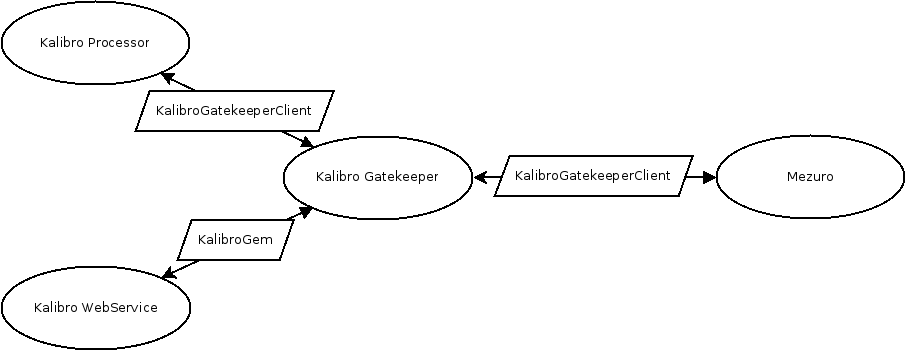
\includegraphics[scale=0.415]{images/mezuro-architecture-actual.png}
    \caption{Arquitetura atual do web-service.}
    \label{fig:architecture-1}
  \end{figure}
  As elipses são os diferentes softwares envolvidos e os paralelogramos as interfaces de comunicação entre eles. Na base do Mezuro existe o Kalibro, que está sendo reescrito
  de Java para Ruby e segmentado em três entidades menores, como ilustrado na imagem a seguir:
  \begin{figure}[H]
    \centering
      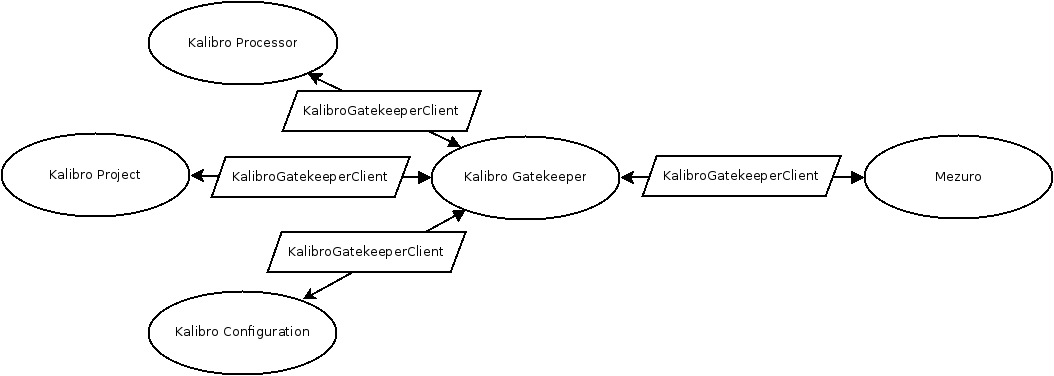
\includegraphics[scale=0.415]{images/mezuro-architecture-predicted.png}
    \caption{Arquitetura futura do web-service.}
    \label{fig:architecture-1}
  \end{figure}
  O objetivo pretendido com quebra da estrutura monolítica do Kalibro é que sua manutenção e evolução torne-se mais fácil, sem que todo o sistema venha a ser comprometido com tal ação.
  \subsection{Diferenciais} \label{subsec:motivacao}
  As principais motivações para o surgimento de uma ferramenta como o Mezuro são os seguintes problemas:
  \begin{itemize}
      \item Não há parâmetros de comparação consolidados entre projetos
      \item Existem estudos, mas poucos dados empíricos
      \item Ainda é dada pouca importância ao monitoramento de código
  \end{itemize}
  \subsection{Por que usar o Mezuro?} \label{sec:projeto-mezuro}
  Idealizado como uma plataforma de métricas de código, um dos diferenciais do Mezuro reside na possibilidade de gerar informação sobre o código-fonte de forma contínua: o usuário decide quando analisar novamente o projeto e acompanha detalhadamente a evolução das notas ao longo do tempo. Os resultados de cada análise são públicos, o que permite uma maior transparência entre o desenvolvedor e a comunidade que utiliza aquele software, esta, que por meio dos resultados das métricas providas pelo Mezuro, pode decidir se aquela solução atende ou não às suas necessidades e se deve depositar confiança na qualidade do software desenvolvido.
  \subsection{Principais funcionalidades}\label{sec:princ-funcionalidades}
  No Mezuro, as funcionalidades podem ser divididas em dois grupos:
  \begin{itemize}
    \item Projeto
      \begin{itemize}
      \item Download do código-fonte a partir de repositórios (Git, Subversion, Bazaar etc) ou via arquivo compactado
          \item Escolha da periodicidade do processamento do código (1 dia, 2 dias, semanal, quinzenal e mensal)
          \item Escolha de qual configuração de métricas cada repositório irá utilizar
          \item Nota de cada métrica da configuração para cada arquivo do repositório
          \item Análise gráfica de cada arquivo do repositório por meio de um gráfico de pontos com notas ao longo do tempo
          \item Resultados públicos e acessíveis à comunidade
      \end{itemize}
      \item Configuração
      \begin{itemize}
      \item Criação de configuração e a possibilidade de clonar de outros usuários
          \item Estatísiticas sobre as configurações mais populares dentro da comunidade
          \item Criação de intervalos qualitativos associados aos valores das métricas
          \item Criação de grupos de leitura para a interpretação textual dos resultados das métricas
          \item Combinações de métricas nativas para criação de análises compostas e mais complexas
      \end{itemize}
  \end{itemize}
  \subsection{A rede social}\label{sec:user-potencial}
  O Mezuro se apresenta para seus usuários no formato de uma rede social, no qual os participantes podem ver a produção de terceiros por meio da avaliação dos projetos ou do clone das configurações. O modelo de rede social foi pensado para que uma comunidade de programadores possa interagir entre si: mesmo que um dado usuário tenha experiência em métricas de software este sempre pode se basear no trabalho de outros usuários. Essa interação mútua e aberta pode ser interessante para desenvolvedores, gerentes de projeto, auditores de software e até mesmo uma equipe de desenvolvimento inteira. O objetivo final é criar uma comunidade que veja o valor de tais metodologias e como isso pode contribuir para o sucesso do seu projeto.
  \subsection{Casos de uso}
  Apresentaremos a seguir as duas principais funcionalidades da ferramenta ilustradas por meio de capturas de telas. Sempre supondo que já se está em uma conta cadastrada no sistema (único privilégio necessário para realizá-las).
    \subsubsection{Criação de configuração}
    \begin{figure}[H]
      \centering
      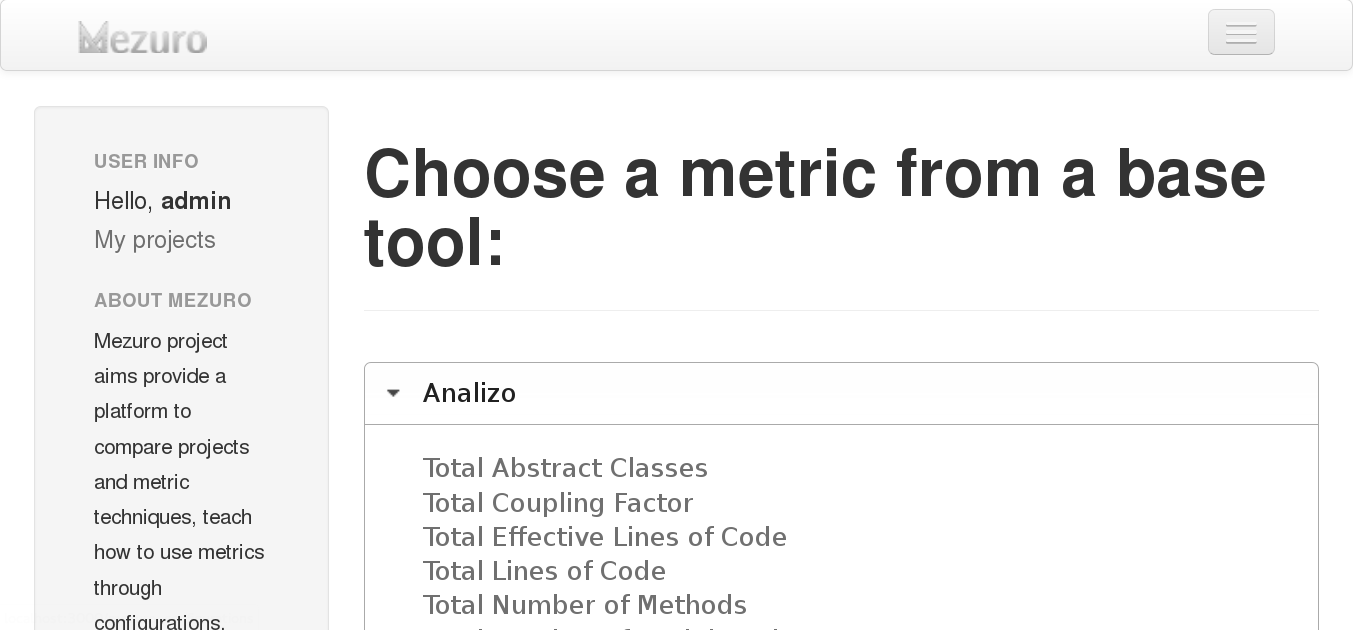
\includegraphics[scale=0.31]{images/choose-metric.png}
      \caption{Interface para escolha de ferramenta extratora de métrica e escolha de uma métrica nativa para adicionar a uma configuração.}
      \label{fig:choose-metric}
    \end{figure}
    Criar uma configuração envolve 5 telas do sistema em 4 passos básicos:
    \begin{enumerate}
      \item Acessar a página de listagem de configurações
      \item Clicando em ``New configuration'', preencher o formulário de criação de configuração e salvá-lo
      \item Clicando em ``Add metric'', escolher a ferramenta de extração e qual métrica a ser usada
      \item Preencher o formulário (detalhado a seguir) e salvá-lo
    \end{enumerate}
    Os passos 3 e 4 devem ser repetidos para cada métrica que for ser adicionada à configuração. O formulário de métrica (passo 4) é complexo se comparado ao de configuração, mas, assim como os demais, cada campo possui detalhes sobre sua utilização. Aqui, destacamos os dois que consideramos os menos óbvios:
    \begin{itemize}
      \item \textbf{Aggregation Form:} Por exemplo, dado um diretório com diversos arquivos contidos, como sua nota será calculada (média, mediana, máximo, etc)
      \item \textbf{Reading Group:} Conjunto de intervalos usado para dar significado prático à nota calculada
    \end{itemize}
    \subsubsection{Criação de projeto e avaliação de repositório}
    Criar um projeto envolve 2 passos básicos:
    \begin{enumerate}
      \item Acessar a página de listagem de projetos
      \item Clicando em ``New project'', escolher o nome, a descrição e salvá-lo
    \end{enumerate}
    \begin{figure}[H]
      \centering
      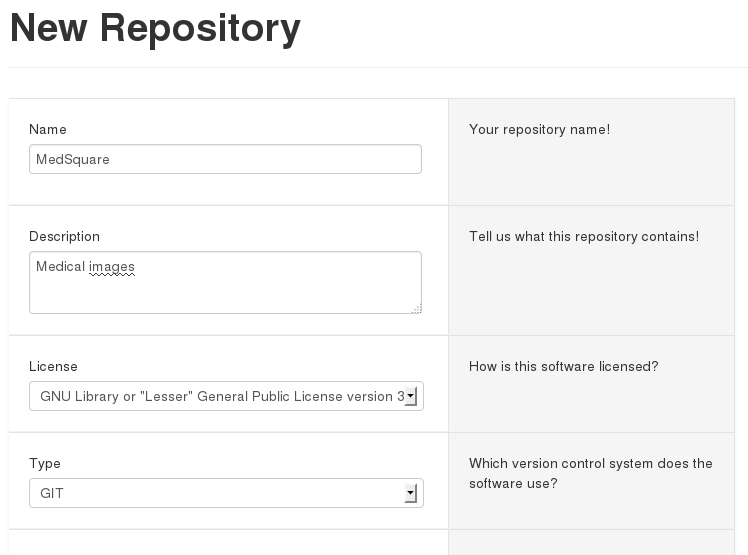
\includegraphics[scale=0.49]{images/new-repository.png}
      \caption{Interface para criação de um novo repositório.}
      \label{fig:choose-metric}
    \end{figure}

    Clicando em ``New repository'' entramos na criação do repositório a ser avaliado. Alguns campos merecem destaque:
    \begin{itemize}
      \item\textbf{Type:} Tipo do repositório (também pode ser um zip ou tarball) onde o código está hospedado
      \item\textbf{Address:} Endereço do repositório remoto ou o caminho absoluto no sistema de arquivos
      \item\textbf{Process Period:} Periodicidade com a qual o código deve ser analizado pela ferramenta (diariamente, semanalmente etc)
      \item\textbf{Configuration:} Configuração de métricas que o usuário deseja utilizar para medir o código (pode ser escolhida dentre todas as configurações criadas pelos usuários)
    \end{itemize}
    Após preencher todos os campos e salvar o repositório, seu primeiro processamento será automaticamente ativado e o usuário será redirecionado para a página que exibe os resultados. Nela, este poderá conferir dados do processamento (tempo gasto para o término de cada uma de suas fases) e navegar na árvore de módulos (pacotes e classes, basicamente) gerada, para que possa visualizar a nota, os resultados das métricas e suas interpretações para cada um deles especificamente. Além disso, ao clicar no nome de uma métrica calculada, um gráfico que representa a evolução dos seus valores ao longo dos processamentos será exibido.

    \begin{figure}[H]
      \centering
      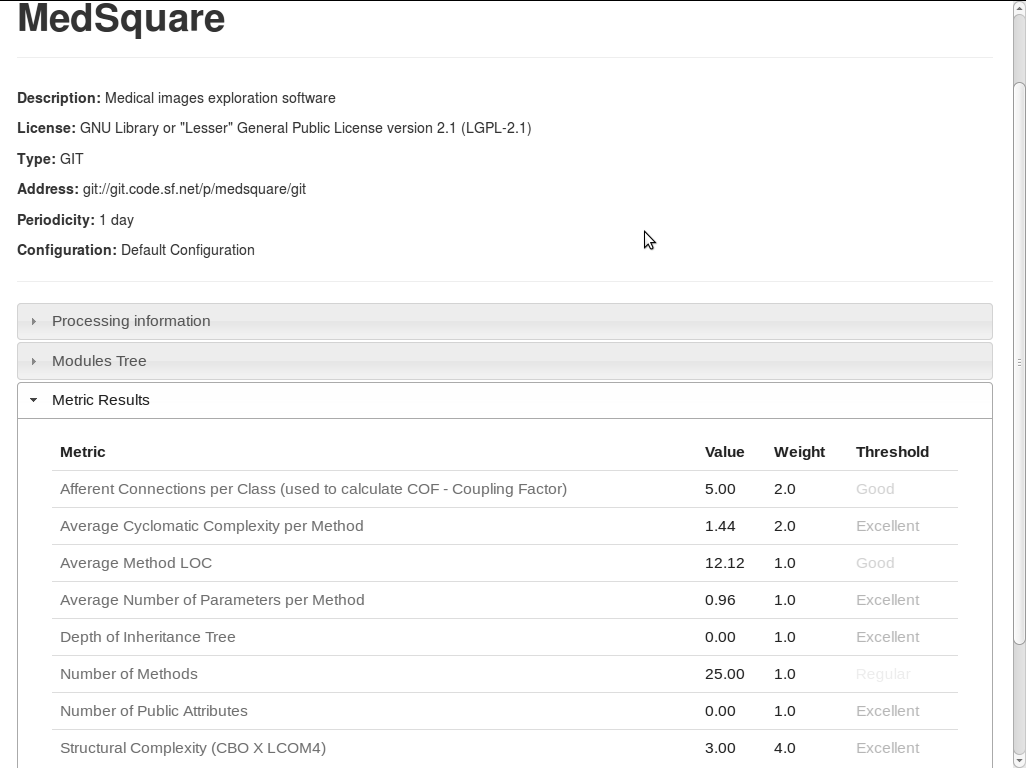
\includegraphics[scale=0.401]{images/new-repository-results.png}
      \caption{Tela de visualização dos resultados do processamento do repositório.}
      \label{fig:choose-metric}
    \end{figure}
\section{Conclusão}
O Mezuro surge como uma potencial resposta para a falta de monitoramento e padronização de código-fonte e a necessidade de avaliação do mesmo, considerando que é um software livre, altamente customizável, com suporte para muitas linguagens computacionais, interface amigável, que fornece histórico de processamentos e também com uma arquitetura planejada para incorporar novas funcionalidades.
\newpage
\bibliographystyle{sbc}
\bibliography{mezuro}
\end{document}
